\chapter{Features and correspondence}
\label{ch:features}

Everything so far assumed that we know which pixel in one image shows
the same landmark as which pixel in another: the data association hidden
in the index $j$ of $\z_{kj}$. Producing those correspondences is the
job of the visual \emph{front-end}, and it is where most of the
engineering of a real system goes. This chapter builds the classical
front-end from its mathematical core. A single matrix, the structure
tensor, tells us which image points can be localised at all. Binary
descriptors make points recognisable across views. Lucas--Kanade
tracking is Gauss--Newton applied to image patches. And RANSAC removes
the wrong correspondences that remain, with a cost that follows from one
line of probability. Along the way we meet the specific way grass breaks
this machinery: not the way one might expect.

\section{Which points can be localised?}

Let $I:\R^2\to\R$ be an image (intensity as a function of the pixel
coordinates $\vect{x}=(u,v)$), and $w\ge0$ a window function centred on
a candidate point, typically a Gaussian.

\begin{proposition}{Local autocorrelation and the structure tensor}{stensor}
The weighted sum of squared differences between the window and a copy
shifted by $\vect\Delta$,
\[
E(\vect\Delta)=\sum_{\vect{x}}w(\vect{x})\bigl(I(\vect{x}+\vect\Delta)
-I(\vect{x})\bigr)^2,
\]
satisfies $E(\vect\Delta)=\vect\Delta\T M\vect\Delta+o(\norm{\vect\Delta}
^2)$, where
\[
M=\sum_{\vect{x}}w(\vect{x})\,\nabla I(\vect{x})\nabla I(\vect{x})\T
=\begin{pmatrix}\sum wI_u^2&\sum wI_uI_v\\\sum wI_uI_v&\sum wI_v^2
\end{pmatrix}
\]
is the \emph{structure tensor}. If $0\le\lambda_{\min}\le\lambda_{\max}$
are its eigenvalues, then to second order
$\min_{\norm{\vect\Delta}=\epsilon}E=\lambda_{\min}\epsilon^2$ and
$\max_{\norm{\vect\Delta}=\epsilon}E=\lambda_{\max}\epsilon^2$.
\end{proposition}

\begin{proof}
By Taylor's theorem, $I(\vect{x}+\vect\Delta)-I(\vect{x})=\nabla I(
\vect{x})\T\vect\Delta+o(\norm{\vect\Delta})$, so each squared term is
$\vect\Delta\T\nabla I\nabla I\T\vect\Delta+o(\norm{\vect\Delta}^2)$,
and summing with the weights gives $\vect\Delta\T M\vect\Delta$. $M$ is
a nonnegative combination of positive semidefinite rank-one matrices,
hence positive semidefinite. For $\norm{\vect\Delta}=\epsilon$, the
Rayleigh quotient $\vect\Delta\T M\vect\Delta/\epsilon^2$ ranges exactly
over $[\lambda_{\min},\lambda_{\max}]$.
\end{proof}

\begin{inwords}
A point can be pinned down only if its neighbourhood changes when moved
in \emph{every} direction. In a flat region nothing changes
($\lambda_{\max}\approx0$). On an edge, moving along the edge changes
nothing ($\lambda_{\min}\approx0$): you can tell you are on the edge, not
where. At a corner both eigenvalues are large. The smaller eigenvalue is
therefore the natural ``cornerness''; it measures how badly the point
can be confused with its own shifted copy.
\end{inwords}

\begin{definition}{Corner detectors}{corners}
With $M$ computed with a Gaussian window at every pixel:
\begin{itemize}[nosep]
\item \emph{Shi--Tomasi}: response $\lambda_{\min}(M)$;
\item \emph{Harris}: response $\det M-k(\tr M)^2=\lambda_{\min}
  \lambda_{\max}-k(\lambda_{\min}+\lambda_{\max})^2$, $k\approx0.04$,
  which avoids the square root of the eigenvalue formula;
\item \emph{FAST}: $p$ is a corner if, on the 16-pixel circle of radius
  3 around it, at least $n$ ($9$ or $12$) contiguous pixels are all
  brighter than $I(p)+t$ or all darker than $I(p)-t$. Most pixels are
  rejected after testing a handful of circle pixels, which makes FAST
  very cheap; ORB then ranks FAST corners by their Harris response.
\end{itemize}
Keypoints are the local maxima of the response, above a threshold, kept
at a minimum distance from each other (non-maximum suppression).
\end{definition}

\begin{figure}[ht]
\centering
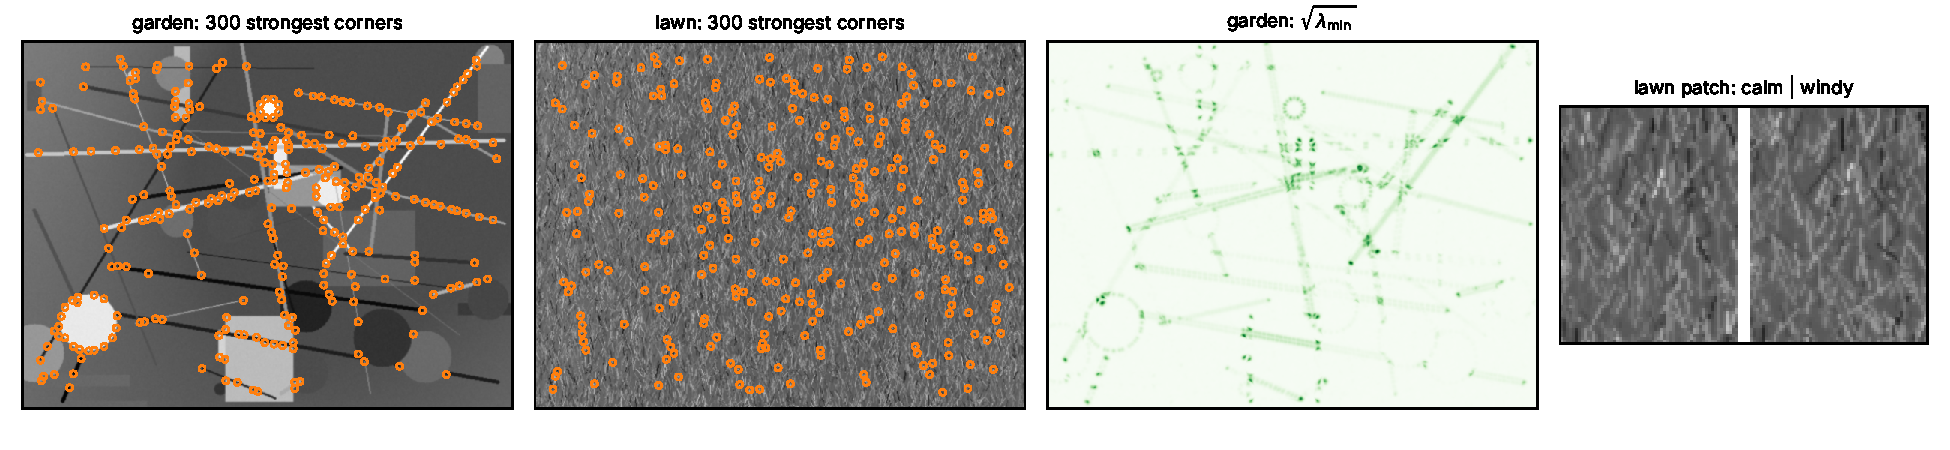
\includegraphics[width=\linewidth]{figures/ch05_textures.pdf}
\caption{The two synthetic textures used in this chapter. The garden's
corners concentrate on the man-made shapes; the lawn has corners
everywhere. Third panel: the Shi--Tomasi response of the garden, high
only at corners. Right: a patch of lawn before and after a gust of wind
that rotates each blade about its root by $\sim11^\circ$.}
\label{fig:textures}
\end{figure}

\section{Recognising a point: binary descriptors}

A keypoint must be found again in another image taken from elsewhere,
at another time. We attach to it a \emph{descriptor}, a vector that
summarises its neighbourhood and changes little under the viewpoint and
lighting changes we expect.

\subsection{Orientation}

\begin{proposition}{The intensity centroid is covariant}{centroid}
For a keypoint at the origin and the disc $D$ of radius $r$ around it,
let $m_{pq}=\int_Du^pv^qI(u,v)\,\mathrm du\,\mathrm dv$ and
$\theta=\operatorname{atan2}(m_{01},m_{10})$. If the image is rotated
about the keypoint by $\alpha$, $I'(\vect{x})=I(R_\alpha^{-1}\vect{x})$,
then $\theta'=\theta+\alpha$ (modulo $2\pi$, when $(m_{10},m_{01})\neq
\vect0$).
\end{proposition}

\begin{proof}
Write $\vect{c}=(m_{10},m_{01})=\int_D\vect{x}\,I(\vect{x})\,
\mathrm d\vect{x}$. With the substitution $\vect{x}=R_\alpha\vect{y}$,
which maps $D$ onto itself and has unit Jacobian,
\[
\vect{c}'=\int_D\vect{x}\,I(R_\alpha^{-1}\vect{x})\,\mathrm d\vect{x}=
\int_DR_\alpha\vect{y}\,I(\vect{y})\,\mathrm d\vect{y}=R_\alpha\vect{c}.
\]
Rotating a vector by $\alpha$ adds $\alpha$ to its polar angle.
\end{proof}

The disc matters: a square window is not mapped onto itself by a
rotation, and the property would only hold approximately. On pixels the
integral becomes a sum and the identity holds up to interpolation
error.

\subsection{BRIEF}

\begin{definition}{Steered BRIEF}{brief}
Let $I_s$ be the image smoothed by a Gaussian, and
$(\vect{a}_k,\vect{b}_k)$, $k=1,\dots,256$, a fixed pattern of point
pairs drawn once and for all from an isotropic Gaussian inside a
$31\times31$ patch. The descriptor of a keypoint $\p$ with orientation
$\theta$ is the bit string
\[
\beta_k=\bigl[\,I_s(\p+R_\theta\vect{a}_k)<I_s(\p+R_\theta\vect{b}_k)
\,\bigr],\qquad k=1,\dots,256,
\]
and descriptors are compared by the Hamming distance (the number of
differing bits), computed with an exclusive-or and a population count.
\end{definition}

Two properties make BRIEF attractive on a small computer. It is cheap:
256 comparisons to build, 32 bytes to store, a few machine instructions
to compare. And it is invariant to any affine change of brightness
$I\mapsto aI+b$ with $a>0$, since smoothing commutes with such a map and
comparisons are preserved by it (Exercise~\ref{ex:5affine}); it is
approximately invariant to any increasing change, such as a gamma
curve. Steering by $\theta$ (\cref{prop:centroid}) adds invariance to
in-plane rotation. ORB, the descriptor of ORB-SLAM, is exactly this
construction plus a scale pyramid and a pattern chosen to decorrelate the
bits.

\subsection{Matching}

\begin{definition}{Matching with the ratio test}{matching}
For each descriptor $\vect{d}$ of image~0, let $\vect{d}_1'$ and
$\vect{d}_2'$ be its nearest and second-nearest neighbours in image~1.
Accept the pair $(\vect{d},\vect{d}_1')$ if
$\mathrm{dist}(\vect{d},\vect{d}_1')<\tau\,\mathrm{dist}(\vect{d},
\vect{d}_2')$ (Lowe's ratio test, $\tau\approx0.8$) and, optionally, if
$\vect{d}$ is also the nearest neighbour of $\vect{d}_1'$ in image~0
(mutual consistency).
\end{definition}

The ratio test asks not ``is the best match good?'' but ``is it clearly
better than the alternative?''. A feature on a repetitive structure has
several near-identical candidates and is rejected even when one of them
is right, which is the behaviour we want: an ambiguous match is worse
than none. The notebook shows the distribution of the ratio for correct
and wrong matches: at $\tau=0.8$ it keeps 87\,\% of the correct nearest
neighbours and 31\,\% of the wrong ones. What survives still contains
errors, which geometry removes (\cref{sec:ransac}).

\begin{figure}[ht]
\centering
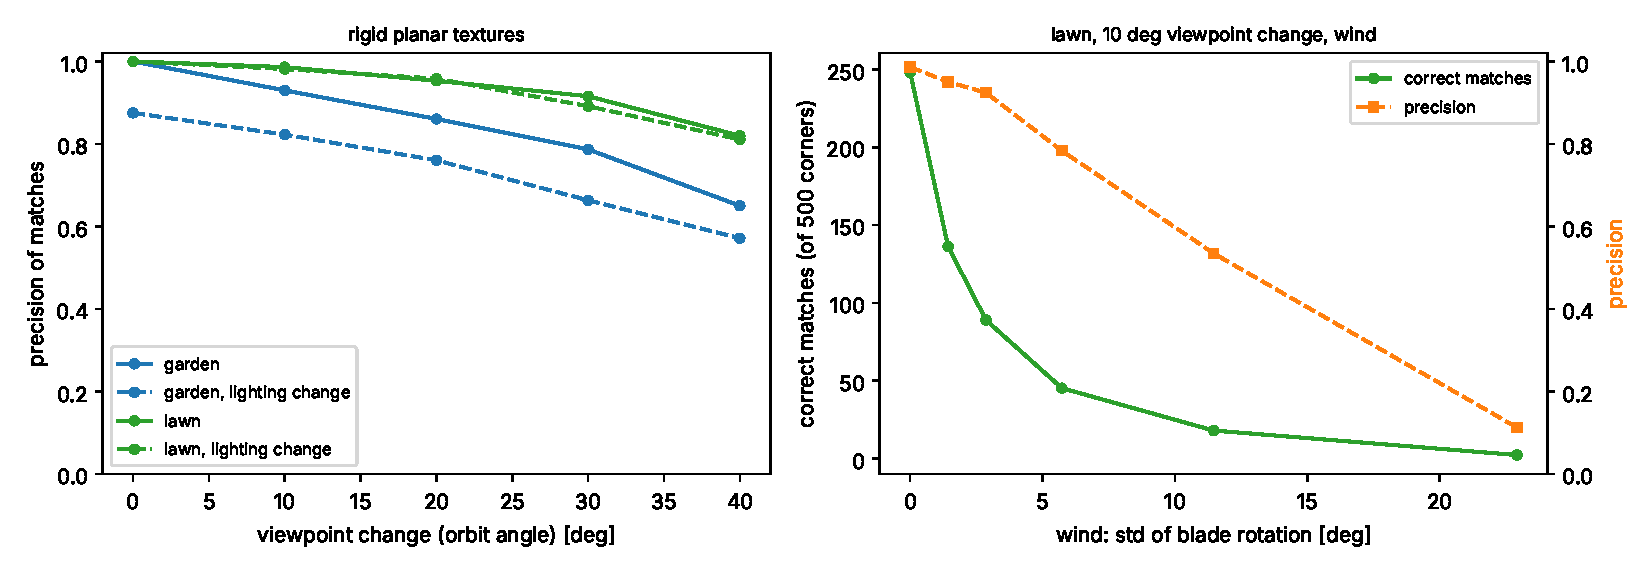
\includegraphics[width=\linewidth]{figures/ch05_matching.pdf}
\caption{Precision of oriented-BRIEF matching (fraction of matches whose
transfer error is below 3\,px; 500 Shi--Tomasi corners per image, ratio
test and mutual check, mean of 4 seeds). Left: rigid planar textures
viewed from an increasingly oblique angle, with and without a change of
lighting. Right: the lawn at a fixed $10^\circ$ change, while wind
rotates each blade about its root by a random angle.}
\label{fig:matching}
\end{figure}

\Cref{fig:matching} holds a surprise. On a rigid plane the lawn matches
\emph{better} than the garden: random blades make every patch unique,
whereas the garden's straight edges and uniform shapes produce
look-alike corners. The difficulty of grass is not its texture. It is
that grass moves. A random rotation of each blade by a few degrees, the
effect of a light breeze or of the mower's own passage, divides the
number of correct matches by three; at $12^\circ$ almost nothing is
left, and what remains is half wrong.

\section{Tracking a point: Lucas--Kanade}

Between consecutive frames of a video, motion is small, and we can track
points instead of re-detecting and matching them.

\begin{proposition}{Lucas--Kanade is Gauss--Newton}{lk}
Let $W$ be a window around a point of $I_0$, and seek the displacement
$\vect{d}$ minimising $E(\vect{d})=\sum_{\vect{x}\in W}\bigl(I_1(
\vect{x}+\vect{d})-I_0(\vect{x})\bigr)^2$ (brightness constancy). One
Gauss--Newton step from $\vect{d}$, with $\nabla I_1(\vect{x}+\vect{d})$
approximated by $\nabla I_0(\vect{x})$, solves
\begin{equation}\label{eq:lk}
M\,\vect\delta=-\sum_{\vect{x}\in W}\nabla I_0(\vect{x})\bigl(I_1(
\vect{x}+\vect{d})-I_0(\vect{x})\bigr),\qquad
M=\sum_{\vect{x}\in W}\nabla I_0\nabla I_0\T,
\end{equation}
the structure tensor of the window (with a box window). The step is
uniquely defined if and only if the gradients in $W$ are not all
parallel; otherwise only the component of the motion along the common
gradient direction is determined (the \emph{aperture problem}).
\end{proposition}

\begin{proof}
The residuals are $r_{\vect{x}}(\vect{d})=I_1(\vect{x}+\vect{d})-I_0(
\vect{x})$, with Jacobian rows $\nabla I_1(\vect{x}+\vect{d})\T\approx
\nabla I_0(\vect{x})\T$. The Gauss--Newton normal equations
\eqref{eq:gn} are then \eqref{eq:lk}. $M$ is singular if and only if
there is $\vect{n}\neq\vect0$ with $\vect{n}\T M\vect{n}=\sum(\nabla I_0
\T\vect{n})^2=0$, i.e.\ every gradient in $W$ is orthogonal to
$\vect{n}$, i.e.\ all gradients are parallel. Then the residuals do not
change to first order when $\vect{d}$ moves along $\vect{n}$, so that
component is unobservable.
\end{proof}

\begin{inwords}
The same matrix decides whether a point is a good corner and whether it
can be tracked: Shi and Tomasi called their detector ``good features to
track'' for exactly this reason. Like any Gauss--Newton method,
Lucas--Kanade converges only from close enough: in practice, for
displacements smaller than about half the window. A Gaussian pyramid
extends the range: at level $\ell$ of a pyramid of half-resolution
images a displacement $\vect{d}$ becomes $\vect{d}/2^\ell$; solve at the
coarsest level, double, and refine on the next finer one
(\cref{fig:lk}).
\end{inwords}

\begin{figure}[ht]
\centering
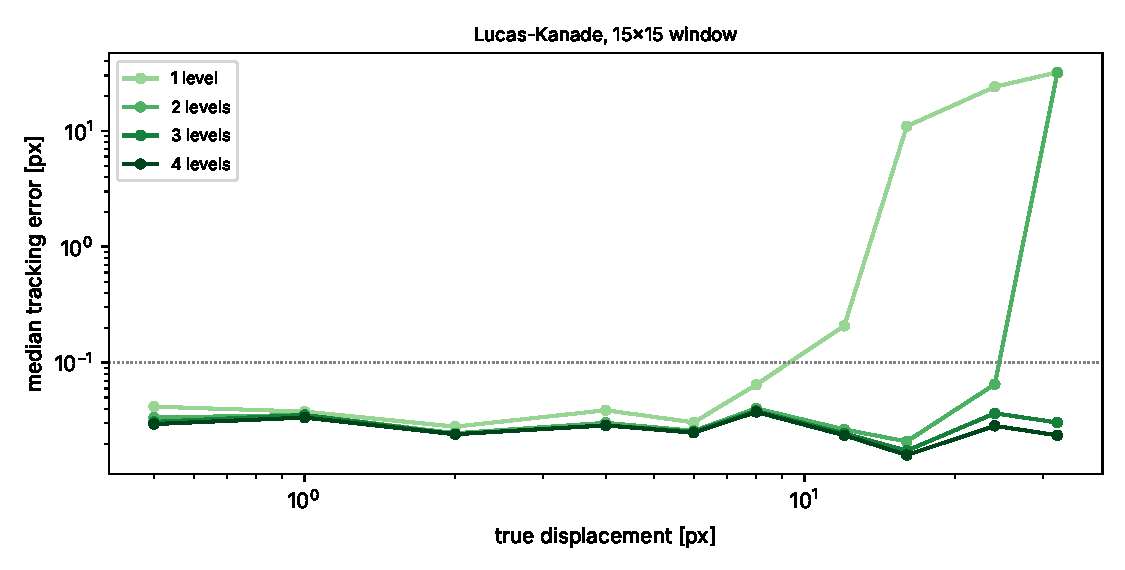
\includegraphics[width=0.75\linewidth]{figures/ch05_lk.pdf}
\caption{Median tracking error of Lucas--Kanade with a $15\times15$
window on the garden texture, for a pure translation of growing size.
A single level fails beyond about 8\,px; four levels reach 32\,px with
the same sub-pixel accuracy.}
\label{fig:lk}
\end{figure}

\section{Removing wrong correspondences: RANSAC}
\label{sec:ransac}

After matching, a fraction $1-w$ of the correspondences is still wrong,
and Chapter~\ref{ch:nls} showed that even robust kernels need a
reasonable starting point. The remedy is to use the \emph{geometry}:
correct correspondences agree on one model (a homography, an essential
matrix, a pose), wrong ones do not.

\begin{definition}{RANSAC}{ransac}
Given $n$ data, a solver that computes a model from a minimal sample of
$s$ data, and an inlier threshold $t$: repeat $N$ times: draw $s$ data
at random, fit the model, and count the data whose residual is below $t$
(its \emph{consensus set}). Keep the model with the largest consensus
set, then refit it on all its inliers.
\end{definition}

\begin{proposition}{How many samples?}{ransacN}
If a fraction $w$ of the data are inliers and samples are drawn
independently, a sample is outlier-free with probability $w^s$ (for
large $n$), and $N$ samples contain at least one outlier-free sample
with probability at least $p$ as soon as
\begin{equation}\label{eq:ransacN}
N\ \ge\ \frac{\log(1-p)}{\log(1-w^s)} .
\end{equation}
\end{proposition}

\begin{proof}
Drawing with replacement, each of the $s$ data is an inlier with
probability $w$, independently, so the sample is clean with probability
$w^s$ (without replacement the probability is $\prod_{i<s}\frac{wn-i}
{n-i}$, which tends to $w^s$ as $n\to\infty$). The $N$ samples are
independent, so all are contaminated with probability $(1-w^s)^N$. We
need $(1-w^s)^N\le1-p$; take logarithms, both of which are negative.
\end{proof}

\begin{center}
\begin{tabular}{@{}lccc@{}}
\toprule
Model & $s$ & $N$ at $w=0.5$ & $N$ at $w=0.3$\\
\midrule
Pose from 3 points (P3P, Chapter 7) & 3 & 35 & 169\\
Homography & 4 & 72 & 567\\
Essential matrix, five-point (Chapter 6) & 5 & 146 & 1893\\
Fundamental matrix, eight-point (Chapter 6) & 8 & 1177 & 70\,188\\
\bottomrule
\end{tabular}
\end{center}

\begin{inwords}
The cost of RANSAC is exponential in the sample size. That is the whole
reason minimal solvers exist and why the five-point algorithm of
Chapter~6 matters more than its eight-point cousin: at $w=0.3$, which
is not pessimistic on a lawn, it is the difference between about two
thousand hypotheses and seventy thousand. In practice $w$ is unknown,
so $N$ is updated from
the best consensus set found so far (adaptive termination); the notebook
shows that this estimate is slightly pessimistic, so RANSAC draws more
samples than \eqref{eq:ransacN} with the true $w$. The threshold comes
from the noise: for Gaussian pixel noise of standard deviation $\sigma$,
the squared transfer error of an inlier is $\sigma^2$ times a $\chi^2$
variable with 2 degrees of freedom, so $t=2.45\sigma$ keeps 95\,\% of
inliers.
\end{inwords}

\begin{figure}[ht]
\centering
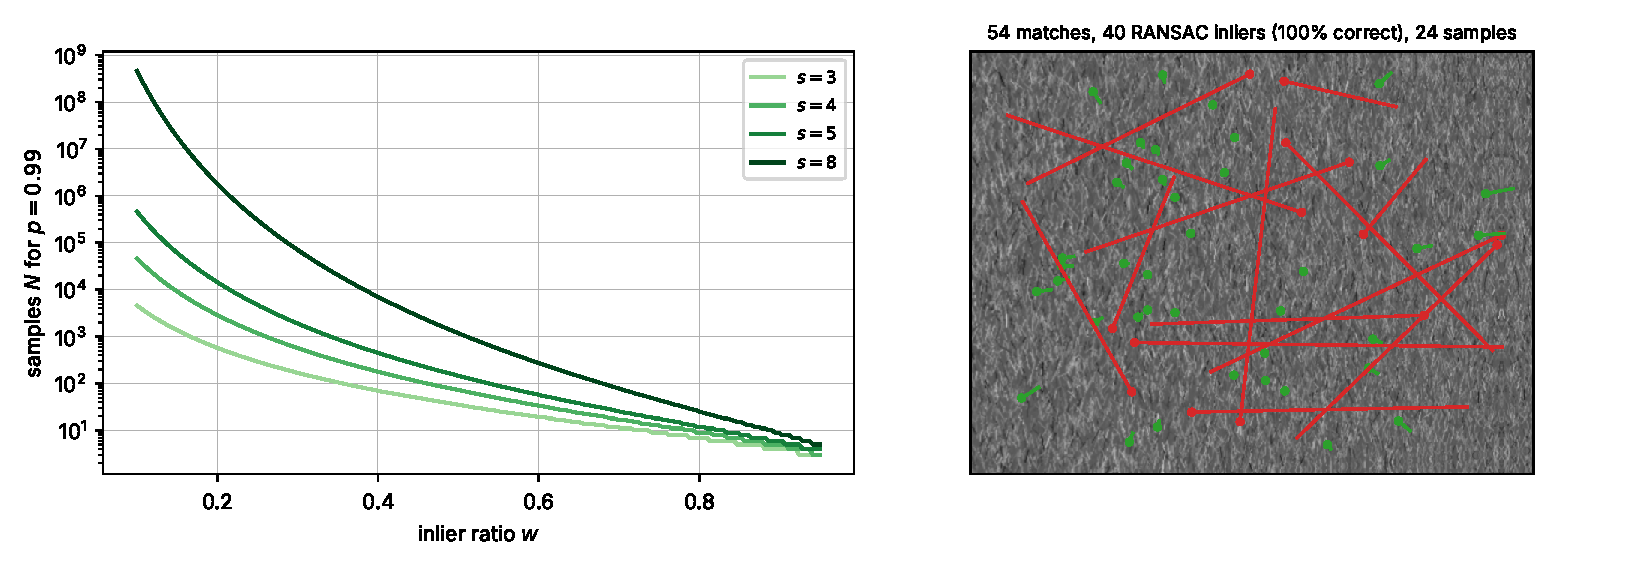
\includegraphics[width=\linewidth]{figures/ch05_ransac.pdf}
\caption{Left: \eqref{eq:ransacN} for $p=0.99$. Right: homography RANSAC
on matches between two views of the lawn with $6^\circ$ of wind; green:
consensus set, all of which are correct; red: rejected matches.}
\label{fig:ransac}
\end{figure}

\begin{mower}
What the experiments say about the mower's front-end:
\begin{itemize}[nosep]
\item \emph{Track, don't re-match, on grass.} Between consecutive frames
  at 20--30\,Hz the blades barely move, and Lucas--Kanade keeps about
  90\,\% of its tracks accurate to a pixel under the same wind that
  divides correct descriptor matches by three (notebook, section 4).
  Matching is for re-finding places seen long ago (Chapter~10), and for
  that, grass is the wrong place to look.
\item \emph{Prefer rigid structure.} Long-term landmarks should be on
  fences, trunks, posts, walls and flower-bed edges. Giving them priority
  (by keeping the best corners per image cell, or by masking the lawn)
  is cheap.
\item \emph{What the simulation leaves out.} Real grass is
  three-dimensional: blades occlude each other and change appearance with
  viewpoint even without wind, and far from the camera its texture falls
  below the pixel size and disappears. Both make things worse than shown
  here; the Rosario dataset and recordings on a real mower will tell by
  how much.
\end{itemize}
\end{mower}

\begin{practice}[\code{vslam/features.py}, \code{vslam/flow.py},
  \code{vslam/ransac.py}, \code{vslam/image.py},
  \code{examples/ch05\_features.py}, \code{notebooks/ch05\_features.ipynb}]
\begin{center}
\begin{tabular}{@{}ll@{}}
\toprule
Code & Formula\\
\midrule
\code{structure\_tensor}, \code{eigenvalues} & \cref{prop:stensor}\\
\code{harris}, \code{shi\_tomasi}, \code{detect} & \cref{def:corners}\\
\code{orientation} & \cref{prop:centroid}\\
\code{describe}, \code{hamming}, \code{match} &
  \cref{def:brief}, \cref{def:matching}\\
\code{flow.lucas\_kanade} & \cref{prop:lk} with a pyramid\\
\code{ransac.ransac}, \code{homography\_ransac} & \cref{def:ransac},
  \eqref{eq:ransacN}\\
\code{image.lawn\_texture}, \code{garden\_texture} & synthetic scenes\\
\bottomrule
\end{tabular}
\end{center}
The tests check the eigenvalue signature of corners, edges and flat
regions; the covariance of the orientation and the rotation invariance
of steered BRIEF under an exact $90^\circ$ rotation; Hamming distances
against a naive count; matching precision under a homography; sub-pixel
LK and the need for a pyramid; \eqref{eq:ransacN}; and homography
RANSAC with 50\,\% outliers. The notebook adds the ratio-test histogram,
the aperture problem, RANSAC's iteration count against the formula,
the lawn in the wind for both matching and tracking, and a comparison
with OpenCV's ORB (which, with its scale pyramid, does better than our
single-scale version on the oblique views).
\end{practice}

\section*{Further reading and C++ pointers}
\addcontentsline{toc}{section}{Further reading and C++ pointers}

C.~Harris and M.~Stephens, ``A combined corner and edge detector'',
1988; J.~Shi and C.~Tomasi, ``Good features to track'', CVPR 1994;
E.~Rosten and T.~Drummond, ``Machine learning for high-speed corner
detection'' (FAST), ECCV 2006; M.~Calonder et al., ``BRIEF: binary
robust independent elementary features'', ECCV 2010; E.~Rublee et al.,
``ORB: an efficient alternative to SIFT or SURF'', ICCV 2011;
B.~D.~Lucas and T.~Kanade, 1981, and S.~Baker and I.~Matthews, ``Lucas--
Kanade 20 years on'', IJCV 2004; M.~A.~Fischler and R.~C.~Bolles,
``Random sample consensus'', CACM 1981. In C++: OpenCV's
\code{ORB}, \code{FastFeatureDetector}, \code{goodFeaturesToTrack},
\code{calcOpticalFlowPyrLK} and \code{findHomography(..., RANSAC)}; the
ORB-SLAM3 extractor adds per-cell quotas to spread features over the
image.

\FloatBarrier
\section*{Exercises}
\addcontentsline{toc}{section}{Exercises}

\begin{enumerate}[label=\textbf{5.\arabic*},ref=5.\arabic*]
\item\label{ex:5harris} Write $r=\lambda_{\min}/\lambda_{\max}$. Show
  that the Harris response is positive exactly when $r$ exceeds a
  threshold depending only on $k$, and compute it for $k=0.04$.
\item\label{ex:5affine} Show that the BRIEF bits are unchanged when the
  image is replaced by $aI+b$ with $a>0$. Why is the invariance only
  approximate for a gamma change $I\mapsto I^\gamma$?
\item\label{ex:5aperture} Let $I_0(u,v)=f(u)$ (vertical stripes) and
  $I_1(\vect{x})=I_0(\vect{x}-\vect{d})$. Compute $M$ in
  \eqref{eq:lk}, and show which component of $\vect{d}$ Lucas--Kanade can
  recover.
\item\label{ex:5ransac} A front-end produces matches with $w=0.4$. How
  many samples does RANSAC need, with $p=0.99$, for $s=5$ and for $s=8$?
  With 30 hypotheses per millisecond, which one fits in a 33\,ms frame?
\end{enumerate}

\subsection*{Solutions}

\textbf{5.1.} Divide by $\lambda_{\max}^2>0$: the response is positive
iff $r-k(1+r)^2>0$, i.e.\ $kr^2-(1-2k)r+k<0$. The roots of this
quadratic are $r_\pm=\bigl(1-2k\pm\sqrt{1-4k}\bigr)/(2k)$, with
$r_-r_+=1$, so on $[0,1]$ the condition is $r>r_-$. For $k=0.04$,
$r_-=0.0436$: Harris accepts a point when its weaker direction carries
at least about 4\,\% of the gradient energy of the stronger one.

\textbf{5.2.} Gaussian smoothing is linear and its kernel integrates to
one, so $(aI+b)_s=aI_s+b$, and $aI_s(\vect{x})+b<aI_s(\vect{y})+b$ iff
$I_s(\vect{x})<I_s(\vect{y})$ when $a>0$. For $g(I)=I^\gamma$,
$g(I)_s\neq g(I_s)$ because smoothing does not commute with a nonlinear
map; but $g$ is increasing, so comparisons between pixels whose
smoothed values are not too close are still preserved, and only bits
from nearly equal pairs can flip.

\textbf{5.3.} $\nabla I_0=(f'(u),0)$, so $M=\begin{pmatrix}\sum f'^2&0
\\0&0\end{pmatrix}$, singular with null direction $(0,1)$. The
right-hand side of \eqref{eq:lk} has a zero second component, so any
$\vect\delta$ with $\delta_u=-\sum f'(I_1-I_0)/\sum f'^2$ solves the
equations: LK recovers $d_u$ (motion across the stripes) and nothing
about $d_v$. The minimum-norm solution sets $\delta_v=0$; our
implementation instead flags the point as untrackable.

\textbf{5.4.} $w^5=0.01024$ gives $N=\lceil\log0.01/\log0.98976\rceil=
448$; $w^8=6.55\times10^{-4}$ gives $N=7025$. At 30 hypotheses per
millisecond the five-point solver needs about 15\,ms, the eight-point
one about 230\,ms: only the minimal solver fits in a frame.
